\chapter{Some concepts of Structural Reliability}
\label{ch:2}
This chapter defines the concept of probability of failure and how it is calculated, and briefly reviews some methods to contextualize the subsequent work. It is based mostly on \citep{Hurtado2013} and \citep{Melchers2018}.\\

\section{Reliability problem formulation}
The reliability problem is based on the performance function $G(\bm{x})$ defined as:
\begin{equation} \label{eq:1}
    G(\bm{x})=R(\bm{x}) - S(\bm{x})
\end{equation}

where $\bm{x}$ is the vector of input variables, in which are included the geometric and material properties, as well as the acting loads, and in general all the variables taken into consideration that affect the behavior of the structure; $S(\bm{x})$ is a load effect acting on the structure, and $R(\bm{x})$ is its capacity to withstand it. The limit state equation corresponds to $G(\bm{x})=0$, i.e. when the acting and resisting forces are equal. A violation of the limite state occurs when $G(\bm{x}) \leq 0$, otherwise (when $G(\bm{x}) > 0$), we say that the structure is safe. \\

For complex problems, the performance function usually cannot be expressed as in \ref{eq:1}, but in the form:

\begin{equation}
    G(\bm{x}) = r(\bm{x}) - \hat{r}
\end{equation}
where $r(\bm{x})$ is an implicit function and $\hat{r}$ is a critical threshold. $r(\bm{x})$ can be, for instance, the result obtained from a finite element analysis. \\

The objective is to determine the probability of failure $p_f$ of the structure:
\begin{equation} \label{eq:pf}
p_f = P[G(\bm{x}) \leq 0]    
\end{equation}

\begin{testexample}[Cantilever beam]
Consider the beam shown in figure \ref{fig:beam}, with rectangular cross section of base $b$ and height $h$. A performance function can be defined as follows:
\begin{equation} \label{eq:example}
    G(\bm{x})=R - \underbrace{\frac{6PL}{bh^2}}_{\sigma_b}
\end{equation}


where $\sigma_b$ is the maximum bending stress to which the beam is subjected and $R$ is the beam resistance. Then we have that if $G(x) \leq 0$, i.e. if $R \leq \sigma_b$, the beam will fail according to this criterion.
\end{testexample}

\begin{marginfigure}[-12\baselineskip]
    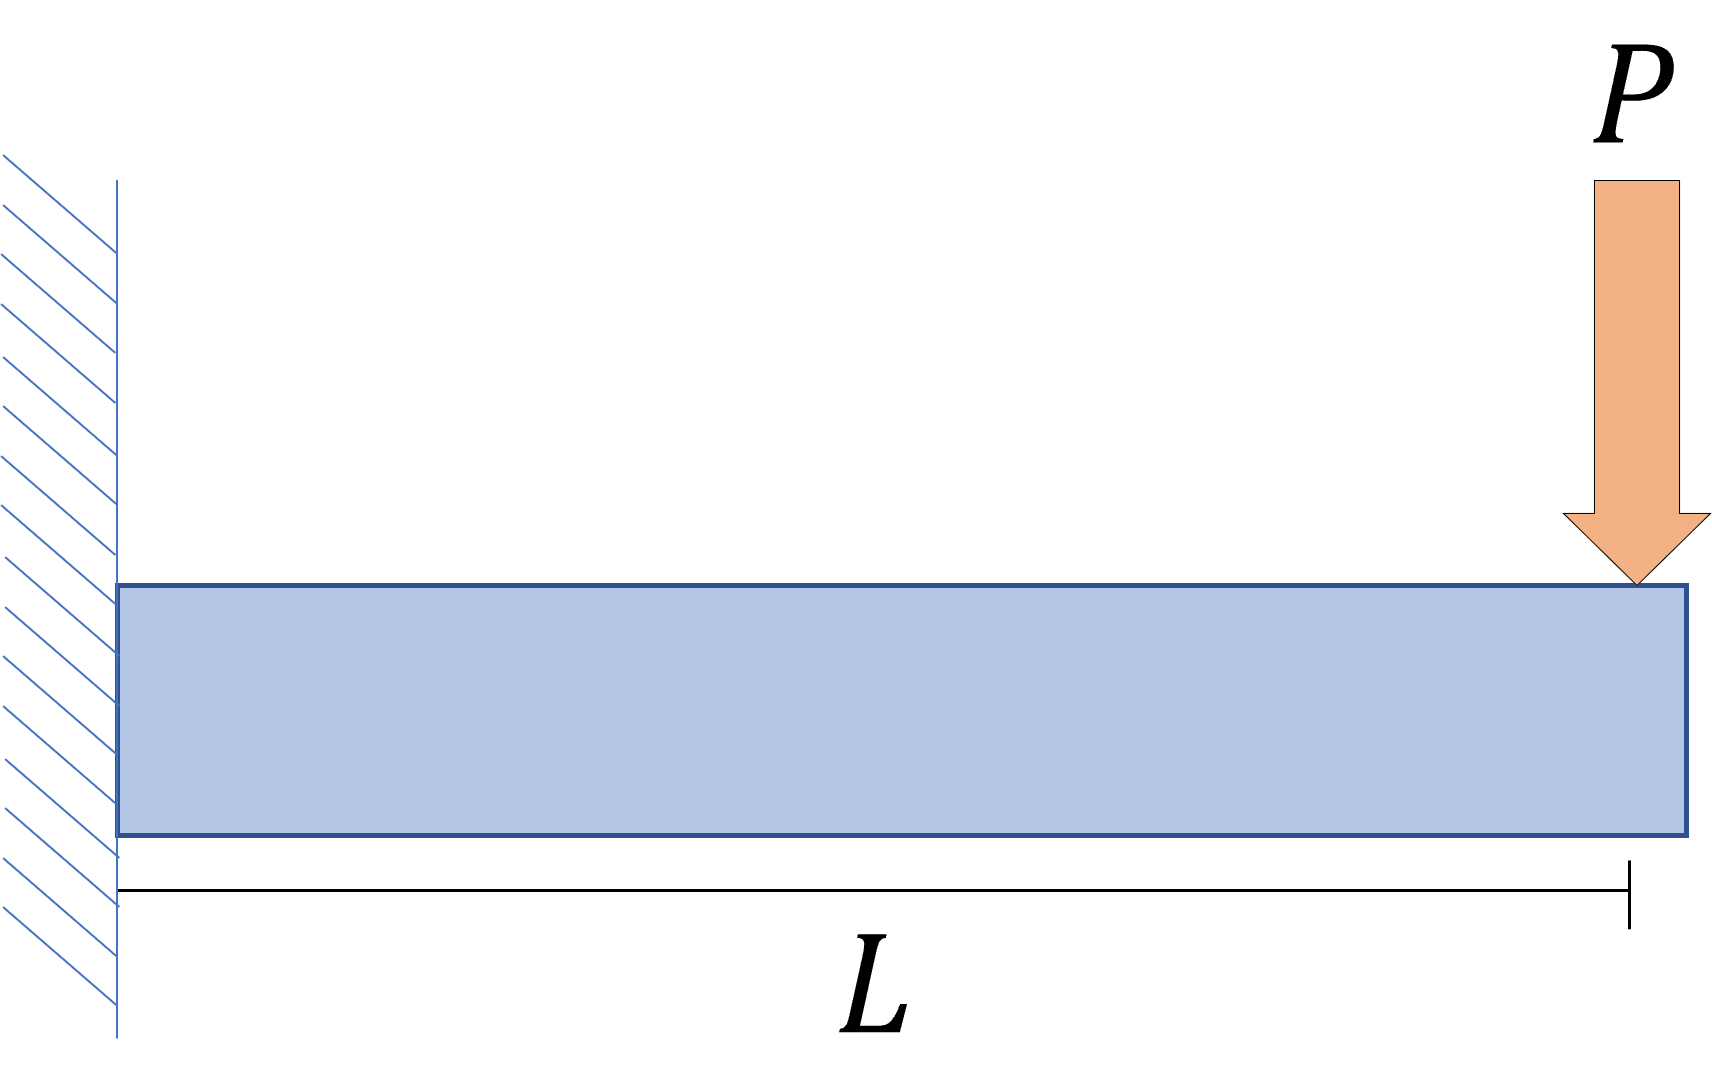
\includegraphics[width=\linewidth]{beam.png}
    \caption{Cantilever beam.}
    \label{fig:beam}
\end{marginfigure}


\section{Realiability assessment approaches}

\subsection{Deterministic approach}
The deterministic approach is the traditional one. In this approach, the uncertainties
in the forces and resistances are covered by assuming that the variation of these
forces and resistances have limits that are not exceeded. Given this simplicity,
it is usually necessary to overestimate the magnitudes in order to provide greater
safety. This is usual in design codes when considering safety factors in the limit
state equations. It is widely used, especially in simple and common problems.
However, this required safety margin implies the need to assume higher costs. \\

In this case, the result of the formula \ref{eq:pf} is either $1$ or $0$, since the values of the variables are considered fixed, thus the inequality is either fulfilled or not.
\begin{testexample}[Cantilever beam (cont.)]
In order to design the beam in such a way that it does not violate the limit state equation considering this approach, design parameters are selected such that $G(\bm{x}) > 0$. For safety reasons, in the equation \ref{eq:example}, $\sigma_b$ is replaced by $\hat{\sigma}_b = \lambda \sigma_b$, being $\lambda \geq 1$ the safety factor, which is determined empirically based on previous experience with similar problems. \\

Although the limit state is not violated, failure may still occur, due to the uncertainty that is ignored.
\end{testexample}
\subsection{Partial probabilistic approach}
The historical record of events that expose structures to large loads, such as
earthquakes, floods, tornadoes, etc., shows that they have a certain frequency
according to their magnitude. For instance, during one day there may be multiple
low-scale earthquakes, but every few years there is one of considerable destructive
power. \\

The partially probabilistic approach handles these return periods when considering
the maximum loads to which a structure will be subjected during certain period of time. This allows the selection of design parameters in accordance with the expected service life of the structure, seeking a balance between the probability of failure and the costs that may be incurred. \\

It can be seen that some randomness is considered when accounting for the variability over time of the loads; however, this approeach does not acknowledge that even at a given instant there is uncertainty.

\begin{testexample}[Cantilever beam (cont.)]
    In this case, to estimate $\hat{\sigma}_b$, the historical records of the values taken by the applied load $P$ are considered to study the frequency of events in which it takes very high values. Then a value of $P$ is selected, attempting to maintain a good balance between the costs and the risk of failure. \\
    
    There is a return period associated with the magnitude of $P$ chosen, which accounts for the probability that the structure will fail during a certain period of time.
\end{testexample}

\subsection{Probabilistic approach}
The variables involved in the performance function can be considered random. For this purpose, through statistical data and experience, the distribution that each of them follows is determined. \\

Let consider the case when $G(\bm{x})$ can be expressed as in \ref{eq:1}. It is possible to obtain probability density functions $f_R(x)$ and $f_S(x)$ that describe $R$ and $S$ respectively. Since the limit state is violated when $G(\bm{x}) \leq 0$, the probability of failure can be roughly represented by the overlap of $f_R(\bm{x})$ and $f_S(x)$ as shown in figure \ref{fig:frfs}. \\

\begin{marginfigure}[-12\baselineskip]
    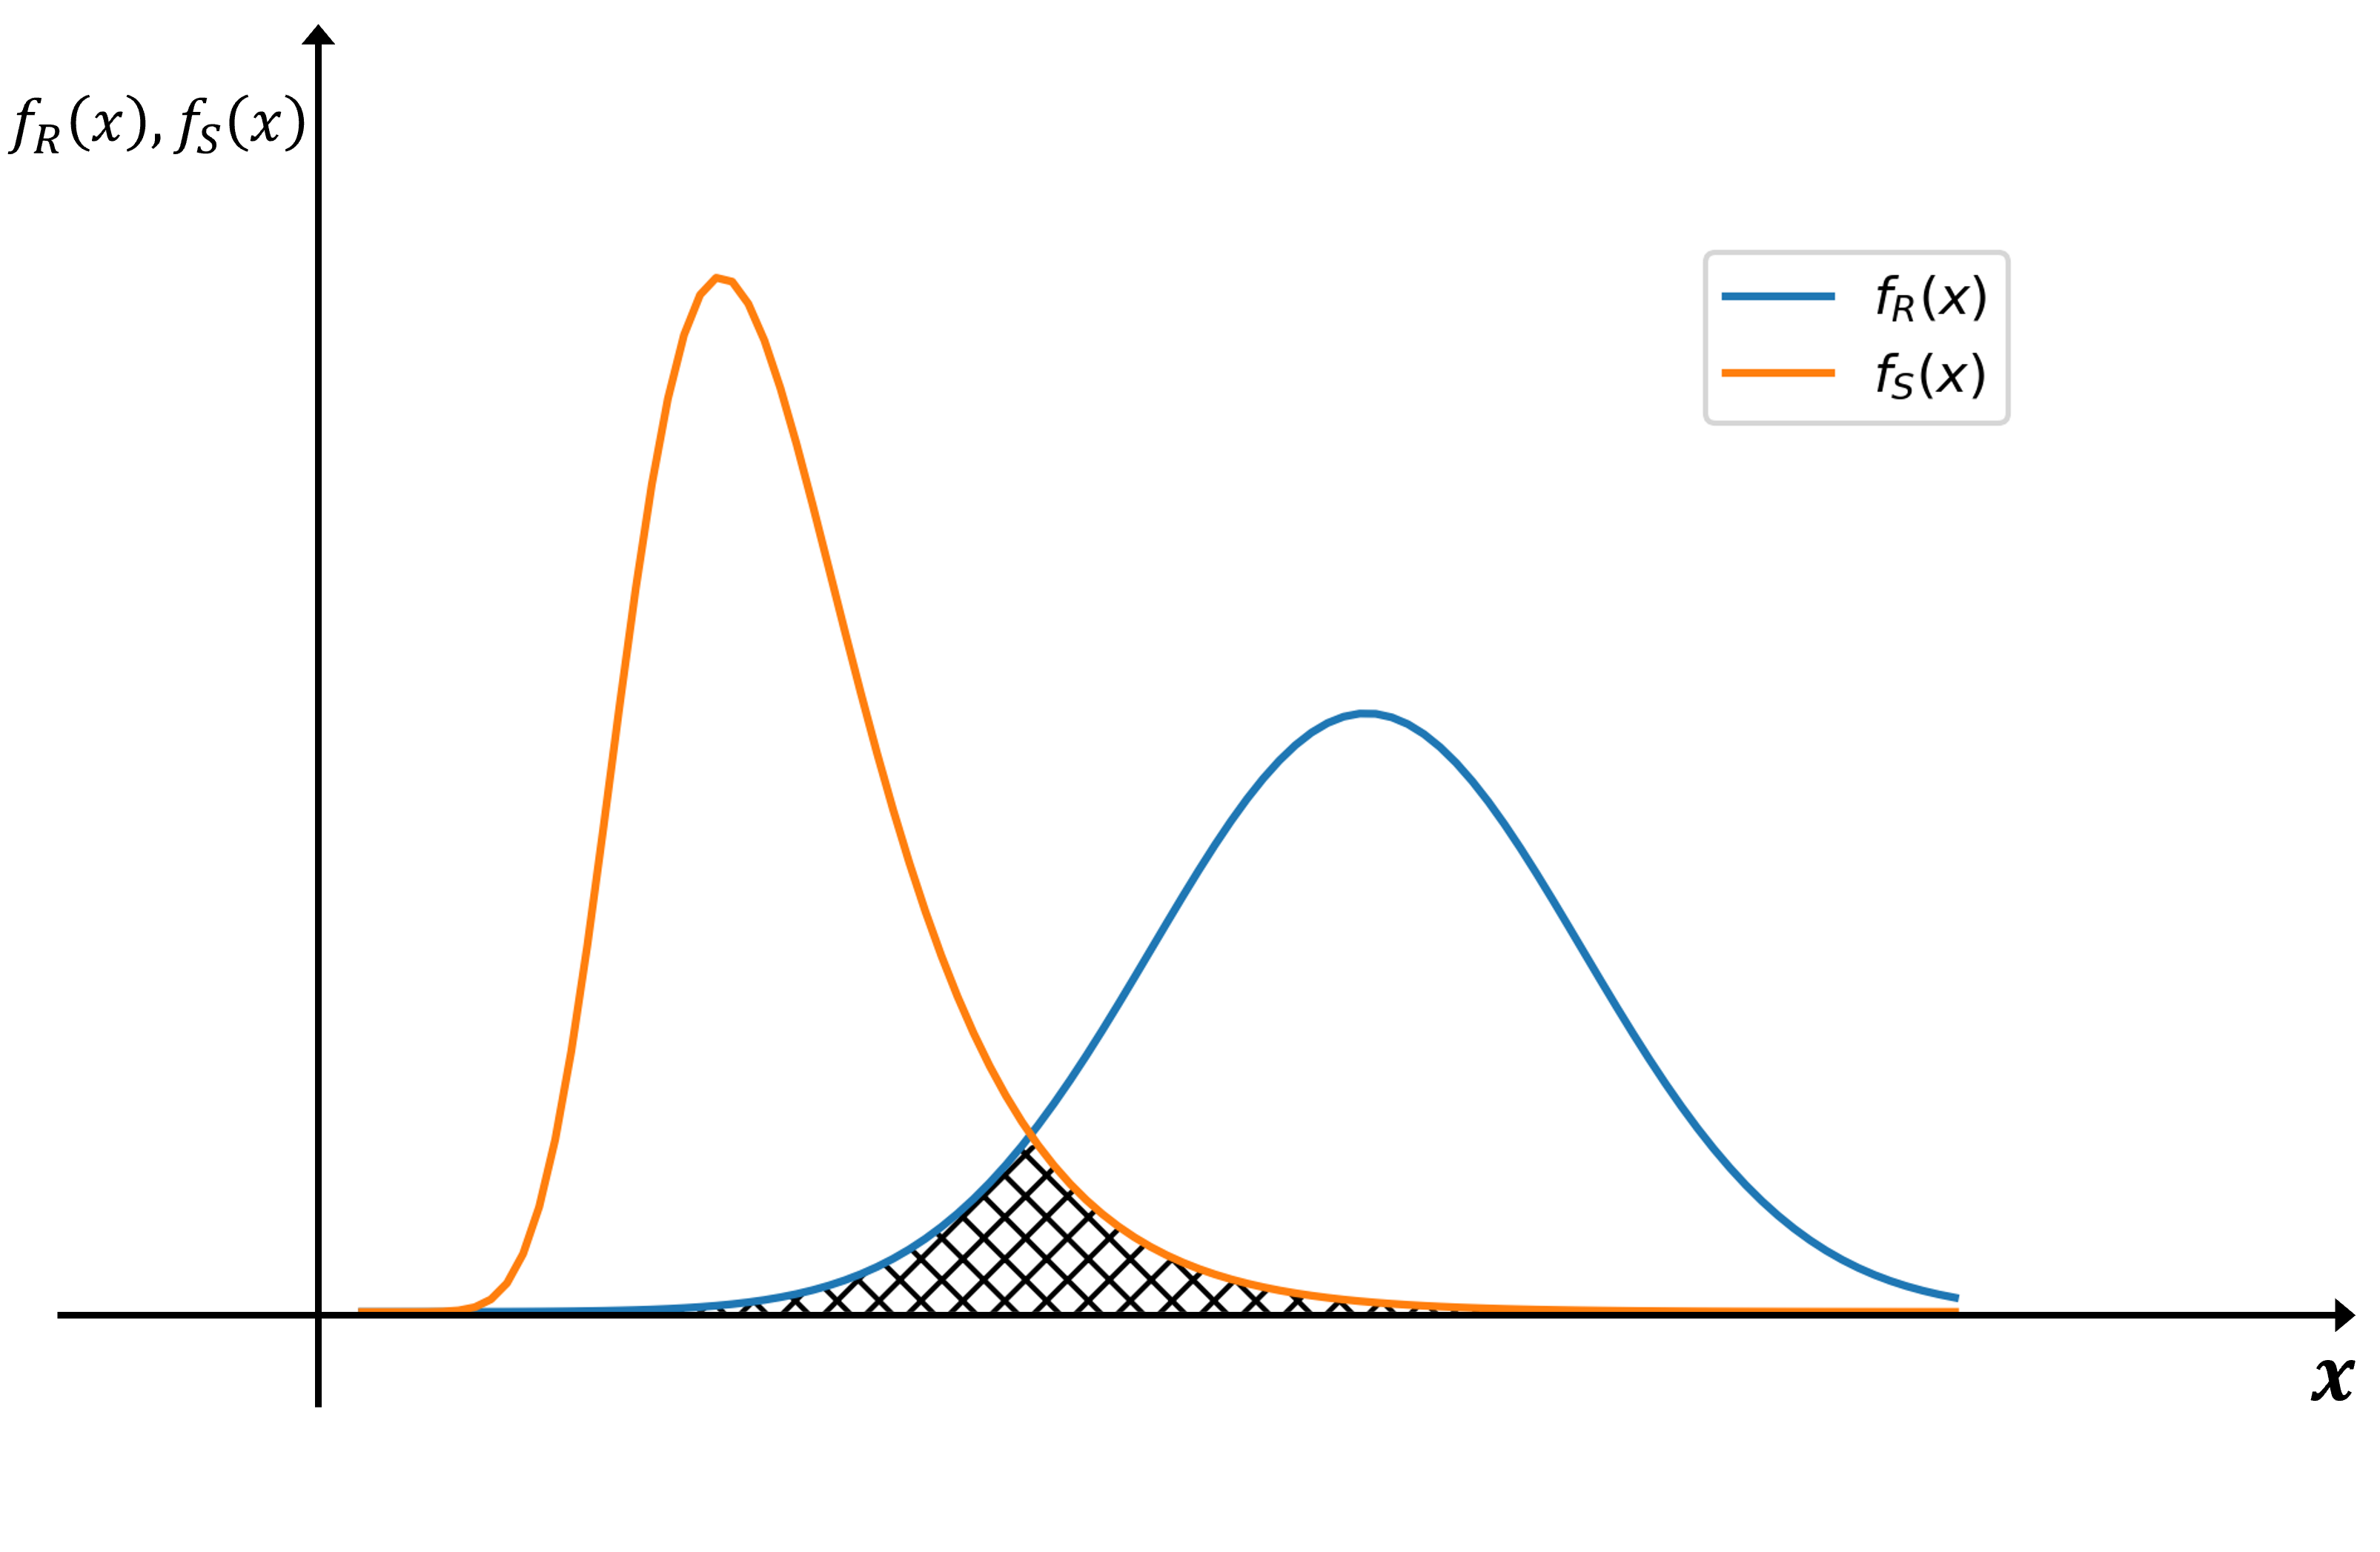
\includegraphics[width=\linewidth]{frfs.png}
    \caption{Representation of $p_f = P\bracket{R(\bm{x}) \leq S(\bm{x})}$}
    \label{fig:frfs}
\end{marginfigure}

When $f_R(x)$ and $f_S(x)$ are independent, the probability of failure can be expressed as:

\begin{equation}
    p_f = \int_{-\infty}^{\infty} F_R(x)f_S(x)\mathrm{d}x
\end{equation}

which is known as a convolution integral, where $F_R(x)$ is the probability that $R \leq x$, so by considering its product with $f_S(x)$ over all possible values of $x$, $p_f$ is obtained. \\

In the general case, the probability of failure is given by:

\begin{equation} \label{eq:pfint}
    p_f = \underset{G(\bm{x})\leq 0}{\int \cdots \int}f_{\bm{x}}(\bm{x})\mathrm{d}\bm{x}
\end{equation}

where $f_{\bm{x}}(\bm{x})$ is the joint probability density function of the considered variables $\bm{x}$. The solution of \ref{eq:pfint} can be tricky. For this purpose, several methods have been developed, some of which will be reviewed in the following section.

\section{Reliabiliy assessment methods}

The analysis methods used to estimate \ref{eq:pfint} can be divided into two main categories: analytic and synthetic. The former are based on the Taylor series expansion of the limit state function, while the latter require the generation of random samples of the variables associated with the model. In this section we will review some generalities of these two categories, their applicability and limitations, with a particular focus on the latter, to which the method reviewed in this document corresponds.

\subsection{Analytic methods (FORM and SORM)}
The \textit{First} and \textit{Second Order Reliability Methods} require the transformation of the vector $\bm{x}$, defined by their joint density function $f_{\bm{x}}$, into a set of normally distributed independent variables $\bm{u}$. The Taylor series expansion of $G(\bm{u})$ is considered, of first order when using FORM, and of second order in the case of SORM. Iteratively, it is obtained the denominated design point $\bm{u^*}$ by minimizing its distance from the origin such that $G(\bm{u^*})=0$. By considering the Taylor series expansion at the design point, a hyperplane is obtained, such that it divides the design space (the possible values taken by the input variables) into the failure and the safe domain. \\

As these methods require the calculation of the gradient of the performance function, in addition to the Hessian matrix in the case of SORM, the practicality of their application depends heavily on the form of the performance matrix, greatly increasing the complexity of the calculations when the dimensionality of the problem increases. \\

\subsection{Synthetic methods (Monte Carlo Simulation)}
Reliability analysis using MCS consists of generating samples in the design space that are used to evaluate the structural model and thus numerically estimate the probability of failure. \\


To generate the sample, random numbers are first generated. Several algorithms have been developed for this purpose, seeking to generate samples uniformly distributed between 0 and 1. Nowadays, the most widely used algorithm is the Mersenne Twister (see \citep{MT}). Starting from the uniformly distributed numbers, the sample is generated following the given distributions. The most general technique for this is the inverse transform method. For some particular distributions there are more efficient methods, for example, for a normal distribution the Box and Muller algorithm (see \citep{BM}) can be used. \\

The equation \ref{eq:pfint} can be written as: 

\begin{equation} \label{eq:pfmc}
    p_f = \int \cdots \int I\bracket{G(\bm{x}) \leq 0}f_{\bm{x}}(\bm{x})\mathrm{d}\bm{x}
\end{equation}

where $I\bracket{G(\bm{x}) \leq 0}$ is an \textit{indicator function} defined as:
\begin{equation}
I\bracket{G(\bm{x}) \leq 0} = 
\begin{cases}
1, \quad \text{if } G(\bm{x}) \leq 0 \\ 
0, \quad \text{if } G(\bm{x}) > 0
\end{cases}
\end{equation}

But equation \ref{eq:pfmc} corresponds to the expected value of $I\bracket{G(\bm{x}) \leq 0}$, so considering a generated sample of $n_{MC}$ elements, being $\bm{\hat{x}}_j$ an element of the sample, it follows that the probability of failure can be approximated as:

\begin{equation}
    p_f \approx \frac{1}{n_{MC}} \sum_{j = 1}^{n_{MC}} I\bracket{G(\bm{\hat{x}_j}) \leq 0}
\end{equation}

This estimated value of $p_f$, since it depends on a random sample, is itself a random variable. A measure of how much its value can vary is the coefficient of variation, which is defined as:

\begin{equation} \label{eq:cov}
    \text{C.O.V}_{p_f} = \sqrt{\frac{1-p_f}{p_f \; n_{MC}}}
\end{equation}

Note that the C.O.V is smaller when the $p_f$ is larger, as the relative variation it can have is smaller; and it can also be reduced by using a larger number of samples. \\

Among the main advantages of MCS is that it makes no assumptions about the limit state function, so it is not necessary to perform any kind of transformation to the design space. In addition, it does not present as many drawbacks as other methods when dealing with high dimensionality problems. However, its main drawback is its computational cost. When having very complex limit state functions, it is necessary to evaluate it too many times to obtain an accurate enough result. Variations of the method are continuously being developed to deal with this problem.The AK-MCS algorithm, which is explained in the next chapter, is one of these variations.
